% Copyright 2013 Nicolai Hähnle <nhaehnle@gmail.com>
%
% This work is licensed under the Creative Commons Attribution-ShareAlike 3.0
% Unported License, see http://creativecommons.org/licenses/by-sa/3.0/
%
% Among other things, this means that yes, you may take e.g. illustrations from
% the book and use them in your own work. However, (a) you must give proper
% attribution by naming me as its original author and (b) you must make your
% derivative work available under the same or similar license terms.
%
% See the Creative Commons website for the exact licensing terms.

\chapter{Dual lattices and Fourier analysis}

Consider the problem of integer programming or, more generally, lattice programming:
given a closed convex set $K$ and a lattice $\Lambda$,
decide whether there exists a lattice point $x \in K \cap \Lambda$.
A natural approach to deciding this problem
is to slice $K$ along translates of a lattice hyperplane,
analogous to the nearest-plane approach to the closest vector problem.
Each of the slices intersecting $K$ leads to an integer programming problem
of lower dimension.
\begin{center}
  \begin{tikzpicture}
    \draw[thick,fill=black!10]
      (0,0) -- (2,-1.3) -- (5,-0.2) node[below right] {$K$} arc[start angle=-50, end angle=10, radius=2cm]
      -- (3,2) -- (1,1.8) -- cycle;

    \draw (6,1.5) node[right] {$y^Tx = \alpha \in \Z$};
    \draw[->] (-0.5,0.1) -- node[left,near end] {$y$} +(0.1,-0.5);
    \clip (-1,-2) rectangle (6,2.5);
    \foreach \t in {-3,-2,-1,0,1,2}
      \draw ($(-1,0) + \t*(0,1.2)$) -- +(7,1.4);
  \end{tikzpicture}
\end{center}
These translates of lattice hyperplanes are defined by equations $y^Tx = \alpha \in \Z$,
where $y \in \R^d$ satisfies $y^Tx \in \Z$ for all $x \in \Lambda$.
This is one justification for the definition of \emph{dual lattices},
which we study in this chapter.

The running time of this particular approach to integer programming
depends strongly on how many lattice hyperplanes intersect $K$.
Fourier analysis neatly relates a lattice and its dual,
which allows us to bound the number of lattice hyperplanes that must be investigated.


\section{The dual lattice}

\begin{definition}
  Let $\Lambda \subset \R^d$ be a full dimensional lattice.
  Its \emph{dual lattice} is given by
  \[
    \Lambda^\star := \{ y \in \R^d ~:~ y^Tx \in \Z \, \forall x \in \Lambda \}
  \]
\end{definition}

\begin{lemma}
  \label{lemma:dual-basis}
  Let $B \in \R^{d \times d}$ be a basis of $\Lambda$.
  Then $\Lambda^\star = \Lambda(B^{-T})$.
  In particular, $\Lambda^\star$ is a lattice.
\end{lemma}
\begin{proof}
  Let $c_1, \ldots, c_d$ be the columns of $B^{-T}$.
  \[
    \begin{array}{|c|}
      \hline \quad c_1^T \quad  \\\hline
      \vdots \\\hline
      c_d^T \\\hline
    \end{array}
    \cdot
    \begin{array}{|c|c|c|}
      \hline  & &\\[0.5em]
      b_1 & \dots & b_d \\
      & & \\[0.5em]\hline
    \end{array}
    =
    \begin{array}{|lcr|}
      \hline 1 & & \\
       & \ddots & \\
      & & 1 \\\hline
    \end{array}
  \]
  Let $y \in \Lambda^\star$.
  Since the $c_1, \ldots, c_d$ form a basis of $\R^d$,
  we can write
  \[
    y = \alpha_1 c_1 + \dots + \alpha_d c_d,\, \alpha_j \in \R
  \]
  It suffices to show that all $c_j \in \Z$,
  which follows from
  \[
    \Z \ni y^T b_j = \alpha_1 c_1^T b_j + \dots + \alpha_d c_d^T b_j = \alpha_j.
  \]
  Now suppose $y \in \Lambda(B^{-T})$, that is,
  we can write
  \[
    y = \alpha_1 c_1 + \dots + \alpha_d c_d,\, \alpha_j \in \Z
  \]
  Let $x \in \Lambda$, that is,
  \[
    x = \beta_1 b_1 + \dots + \beta_d b_d,\, \beta_j \in \Z
  \]
  Then
  \[
    y^Tx = \alpha_1 \beta_1 + \dots + \alpha_d \beta_d \in \Z
  \]
  That is, $y^Tx \in \Z$ for all $x \in \Lambda$,
  hence $y \in \Lambda^\star$ by definition.
\end{proof}

\begin{corollary}
  Let $\Lambda$ be a full-dimensional lattice.
  \begin{enumerate}
    \item $\det \Lambda^\star = \frac{1}{\det \Lambda}$.

    \item $(\Lambda^\star)^\star = \Lambda$.

    \item $(\alpha \Lambda)^\star = \frac{1}{\alpha} \Lambda^\star$ for $\alpha > 0$.
  \end{enumerate}
\end{corollary}

Intuitively, a dense lattice has a sparse dual and vice versa.
Two aspects of this connection are formalized in the Corollary,
but it can also be seen in the lattice hyperplanes corresponding to dual lattice vectors.
For a given $y \in \Lambda^\star$,
the distance between adjacent lattice hyperplanes $y^Tx = \alpha$ and $y^Tx = \alpha + 1$
for $\alpha \in \Z$ is $1 / \|y\|_2$.
In a dense lattice, lattice hyperplane translates must lie close to each other,
which means that dual lattice vectors must be long.
We will develop more statements of this form throughout this chapter.



\section{Successive minima and covering radius}

Let us define some measures of the overall sparsity of a lattice.

\begin{definition}
  Let $\Lambda \subset \R^d$ be a full-dimensional lattice.
  The \emph{successive minima} $\lambda_1, \ldots, \lambda_d$ of $\Lambda$ are
  \[
    \lambda_j(\Lambda) := \min\{ r > 0 ~:~ \dim( \Lambda \cap B(0,r) ) \geq j \}
  \]
  where the dimension is the dimension of the linear span of the lattice points
  of norm at most $r$.

  The \emph{covering radius} of $\Lambda$ is the maximal distance from the lattice:
  \[
    \mu(\Lambda) := \max_{p \in \R^d} d(p, \Lambda)
  \]
  When the lattice is clear from the context,
  we write $\lambda_1, \ldots, \lambda_d$ and $\mu$.
  Furthermore, we write $\lambda_j^\star$ and $\mu^\star$ for the corresponding
  quantities of the dual lattice.
\end{definition}

The covering radius can be equivalently defined as the smallest radius $r$
such that the union of balls of radius $r$ around each lattice point
covers the entire space -- hence its name.

\begin{example}
  \label{example:rect-lattice-minima}
  The lattice $\Lambda := \Lambda \begin{pmatrix} 1 & 0 \\ 0 & 3 \end{pmatrix}$
  satisfies $\lambda_1 = 1$, $\lambda_2 = 3$, and $\mu = \sqrt{10}/2$.
  \begin{center}
    \begin{tikzpicture}
      \foreach \x in {-2,-1,...,2.1}
        \foreach \y in {-1,0,1}
          \fill ($\x*(0.5,0) + \y*(0,1.5)$) circle[radius=2pt];

      \draw (0,0) node[below] {$0$};

      \draw (0.25,0.75) circle[radius=0.76cm];
      \fill (0.25,0.75) circle[radius=2pt] node[right] {$p$};
    \end{tikzpicture}
  \end{center}
\end{example}

As the example shows,
$\lambda_1$ is the length of a shortest vector,
but $\lambda_2$ need not be the length of a ``second-shortest'' vector.
Instead, it is the length of a shortest vector among all vectors that are
linearly independent from a shortest vector.
In general,
we can choose linearly independent vectors $v_1, \ldots, v_d \in \Lambda$ with $\|v_j\|_2 = \lambda_j$.
Such a set of vectors is called a set of \emph{shortest independent vectors} of the lattice.
An exercise shows that such a set need \emph{not} be a basis of the lattice.

\begin{lemma}
  \label{lemma:mu-lambda-d}
  Let $\Lambda$ be a $d$-dimensional lattice.
  Then $\mu \geq \lambda_d / 2$.
\end{lemma}
\begin{proof}
  All lattice points in the interior of the ball of radius $\lambda_d$ around the origin
  lie in a hyperplane $H$.
  A point at distance $\lambda_d/2$ from $H$ has distance at least $\lambda_d/2$ to the lattice,
  see Figure~\ref{fig:mu-vs-lambda-d}.
\end{proof}
\begin{figure}
  \begin{center}
    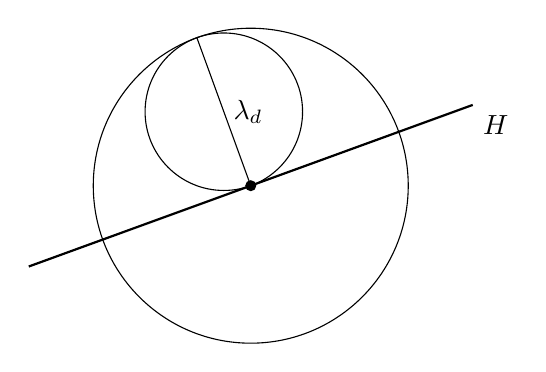
\begin{tikzpicture}
      \fill (0,0) circle[radius=2pt];
      \draw (0,0) circle[radius=2cm];
      \draw[thick] (20:-3) -- (20:3) node[below right] {$H$};

      \draw (0,0) -- node[right] {$\lambda_d$} (110:2);
      \draw (110:1) circle[radius=1cm];
    \end{tikzpicture}
  \end{center}
  \caption{The proof that $\mu \geq \lambda_d / 2$.}
  \label{fig:mu-vs-lambda-d}
\end{figure}

The inequality of this Lemma is tight, as the trivial lattice $\Z$ shows.
Let us now relate quantities of a lattice and its dual.
The following Lemma shows that a lattice and its dual cannot be too dense at the same time.

\begin{lemma}
  \label{lemma:transference-lower-bound}
  Let $\Lambda \subset \R^d$ be a full-dimensional lattice.
  Then $\lambda_1^\star \cdot \lambda_d \geq 1$,
  and hence $\lambda_1^\star \cdot \mu \geq 1/2$.
\end{lemma}
\begin{proof}
  Let $y \in \Lambda^\star$ be a shortest vector
  and let $v_1, \ldots, v_d \in \Lambda$ be shortest independent vectors.
  Since the $v_j$ form a basis of $\R^d$,
  we must have $y^T v_k \neq 0$ for at least one $k$.
  Using the Cauchy-Schwarz inequality and the fact that $y^T v_k \in \Z$,
  we can compute
  \[
    1 \leq |y^T v_k| \leq \|y\|_2 \|v_k\|_2 = \lambda_1^\star \lambda_k \leq \lambda_1^\star \lambda_d \qedhere
  \]
\end{proof}

\begin{example}
  Consider $\Lambda = \Lambda \begin{pmatrix} 1 & 0 \\ 0 & M \end{pmatrix}$ for $M > 1$.
  We have $\Lambda^\star = \Lambda \begin{pmatrix} 1 & 0 \\ 0 & M^{-1} \end{pmatrix}$
  and therefore
  \begin{align*}
    \lambda_1 &= 1 \\
    \lambda_d &= M \\
    \lambda_1^\star &= M^{-1} \\
    \lambda_d^\star &= 1
  \end{align*}
  That is, the inequality of Lemma~\ref{lemma:transference-lower-bound} is tight,
  both when applied to $\Lambda$ and when applied to $\Lambda^\star$.
\end{example}

We would like to have an analogous statement showing
that a lattice and its dual cannot be too sparse at the same time.
That is, we would like to have an \emph{upper bound} on a product of the form $\lambda_1^\star \cdot \lambda_d$.
Some bounds of this type are shown in the exercises
using Minkowski's theorem and LLL-reduced bases.
We will derive a much stronger bound in Section~\ref{sec:transference-bound-banaszczyk}.



\section{Lattice width}

\begin{definition}
  Let $K \subset \R^d$ be a convex body.
  Let $\Lambda$ be a full-dimensional lattice and let $y \in \Lambda^\star$.
  The \emph{lattice width of $K$ with respect to $y$} is
  \[
    w_y(K, \Lambda) := \max_{x \in K} y^T x - \min_{x \in K} y^T x
  \]
  The \emph{lattice width of $K$} is
  \[
    w(K, \Lambda) := \min_{y \in \Lambda^\star \setminus 0} w_y(K,\Lambda)
  \]
  We write $w_y(K)$ or $w(K)$ when the lattice is clear from the context.
\end{definition}



\section{Banaszczyk's transference bound}
\label{sec:transference-bound-banaszczyk}


\section*{Exercises}

\begin{enumerate}
  \item
    Let $\Lambda \subset \R^d$ be a full-dimensional lattice.
    Show: a vector $y \in \Lambda^\star \setminus 0$ is primitive
    if and only if
    every lattice hyperplane $\{ y^T x = \alpha\}$, $\alpha \in \Z$, contains a point of $\Lambda$.

  \item
    Show that the successive minima and the covering radius of a lattice are well-defined,
    i.e. that the minimum (respectively maximum) in the definition is achieved.

  \item
    \begin{enumerate}[(a)]
    \item Show: Every $2$-dimensional lattice has a basis $(b_1, b_2)$
      in which $\|b_1\|_2 = \lambda_1$ and $\|b_2\| = \lambda_2$.

    \item
      Consider the \emph{parity lattice}
      $\Lambda := \{ x \in \Z^d ~:~ x_1 \equiv \dots \equiv x_d \pmod{2} \}$.
      Show: For $d \geq 5$, $\Lambda$ has no basis of shortest independent vectors,
      that is, there is no basis that satisfies $\|b_j\|_2 = \lambda_j$ for all $j$.
    \end{enumerate}

  \item
    Show $\lambda_1^\star \cdot \mu \leq 2^{(d-2)/2}$ using an LLL-reduced basis.

  \item
    \begin{enumerate}[(a)]
      \item Show that
        $\lambda_1 \leq 2 \left( \frac{\det \Lambda}{V_d} \right)^{1/d}$,
        where $V_d = \frac{\pi^{d/2}}{\Gamma(\frac{d}{2} + 1)}$ is the volume of a unit ball.

      \item Show: $\lambda_1 \cdot \lambda_1^\star \leq d$.
    \end{enumerate}

  \item
    Show that lattice width is invariant under linear transformations:
    Let $\Lambda$ be a lattice, $K$ be a convex body, and $f$ a linear transformation.
    Then $w(K, \Lambda) = w(f(K), f(\Lambda))$.

\end{enumerate}

